\textit{This test was made together with Kjeld Jensen in order get one step further to spoofing the drones onboard GPS with an RTK GPS. A ublox Neo6-P GPS and an active anteanna was mounted on a EduQuad drone to obtain the drone's position. A RPI was used on the EDUQuad to convert GPGGA and GPRMC from the Neo6-p GPS to CAN-mesasages.
The test was done by walking 20 meters with the EduQuad two times to compare the output of the UKF with the different GNSS's.
The values used to spoofed the GNSS was found by reading about the ratio between the different DOP-values.
Values available from the Neo6-p GPS, was used directly to spoof the onboard GPS and values not available was either calculated or hardcoded.
This test was also relevant for the indoor flying since the indoor application requires the position of the drone can be spoofed and the accuracies and DOPs can be set}\\

\begin{figure}[H]
\centering
    \includegraphics[width=0.4\textwidth]	{graphics/eduquad_outdoor_flighttest_rpi_can_spoof.png}
	  \caption{Nep-6p connected to a AQ M4 through a RPI using a PEAK-CAN adapter}
    \label{fig:qground_station_dop}
\end{figure}


In order to quickly switch between the onboard GNSS and the Neo-6P GPS during the test, a switch on the Spectrum DX9\footnote{\url{http://www.spektrumrc.com/Products/Default.aspx?ProdId=SPMR9900} last visited 21. Maj} was read in AutoQuad's firmware to decide which of the two GPS's data should be used. When a GPS update(time, position or velocity) is received from the onboard GPS, the struct showed in code \ref{code:gpsData_Struct} is filled in. \\

\begin{lstlisting}[language = c++, caption = Quality checks added to discard bad positions, label=code:gpsData_Struct]
typedef struct {
	...
    double lat;
    double lon;
    float height;   // above mean sea level (m)
    float hAcc;     // horizontal accuracy est (m)
    float vAcc;     // vertical accuracy est (m)
    float velN;     // north velocity (m/s)
    float velE;     // east velocity (m/s)
    float velD;     // down velocity (m/s)
    float speed;    // ground speed (m/s)
    float heading;  // deg
    float sAcc;     // speed accuracy est (m/s)
    float cAcc;     // course accuracy est (deg)
    float pDOP;     // position Dilution of Precision
    float hDOP;
    float vDOP;
    float tDOP;
    float nDOP;
    float eDOP;
    float gDOP;

    //Used in GPS spoof
    uint8_t fix;
    uint8_t satellites;
    int out_cnt;

	...
} gpsStruct_t;
\end{lstlisting}
In order to spoof the onboard GPS correctly, the author and his supervisor decided to overwrite all of the relevant elements in the struct. However, the \ac{RTC} was set from the onboard GPS.

To tell the UKF in AQ how much to believe in the GNSS coordinates, the onboard GPS feeds the UKF with DOP factors. The DOP factors expresses how well the satellites are geometrically placed. If they are all located around the same spot, the DOP factors will be high since the triangulation becomes less accurate. The DOP factors has no unit but is simply a scaling of the error estimate. \cite{kelddueholmmikkellaurentziusannab.o.jensen2015}

 The values listed in table \ref{tab:DOP-values} was used and multiplied by the hDOP received from the Neo-6P GPS. 
The pDOP was set to 1.75 times higher than the hDOP since it incorporates error from both vDOP and hDOP \cite{kelddueholmmikkellaurentziusannab.o.jensen2015}. \\
vDOP is usually 1.5-2 tims higher than hDOP.  \cite{kelddueholmmikkellaurentziusannab.o.jensen2015}. \\
tDOP was sat to 1.5 higher than hDOP since timeerror causes position error. \footnote{\url{http://www.environmental-studies.de/GPS/Dilution-of-precision/dilution-of-precision.html} last visited 22 maj} \\
Since hDOP can be split into nDOP and eDOP, they each have 0.7 of hDOP. \cite{kelddueholmmikkellaurentziusannab.o.jensen2015}

\begin{figure}[H]
\centering
\begin{subfigure}{.5\textwidth}
  \centering
	\label{tab:DOP}
	\begin{tabular}{@{}|l|l|@{}}
	\toprule
	Dop  & Value     \\ \midrule
	{\color{gray}pDOP} & {\color{gray}1.75*hdop} \\ \midrule
	{\color{gray}hDOP} & {\color{gray}1*hdop}    \\ \midrule
	vDOP & 1.5*hdop  \\ \midrule
	tDOP & 1.5*hdop  \\ \midrule
	nDOP & 0.7*hdop  \\ \midrule
	eDOP & 0.7*hdop  \\ \midrule
	{\color{gray}gDOP} & {\color{gray}1*hdop}    \\ \bottomrule
	\end{tabular}
	\caption{Scaling factors used when using Neo-6p GPS. The DOP values grayed out is values not used by AQ directly but gets logged.}
	\label{tab:DOP-values}
\end{subfigure}%
\begin{subfigure}{.5\textwidth}
  \centering
  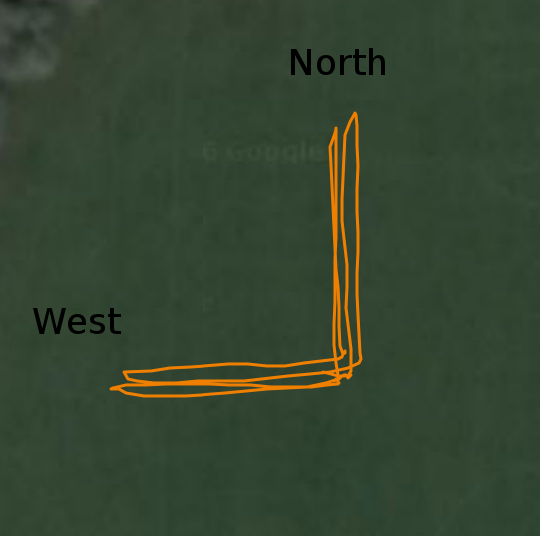
\includegraphics[width=0.75\textwidth]	{graphics/test_walked_90deg.png}
	  \caption{Path walked. If looking closely it can be seen the path was walked twice, once with onboard GPS then using Neo-6p.}
    \label{fig:outdoor_test_walk_90_deg}
\end{subfigure}
	\caption{}
\end{figure}





The test was conducted by walking 20 meters \footnote{Measured by counting footsteps} north, 20 meters south, 20 meters east and 20 meters west. After walking 20 meters a small break of five seconds was held. Figure \ref{fig:outdoor_test_walk_90_deg} shows the walked path.

Figure \ref{fig:outdoor_test_walk_90_deg_x_as_time} shows a plot of the position with x-axix as time.

\begin{figure}[H]
\centering
    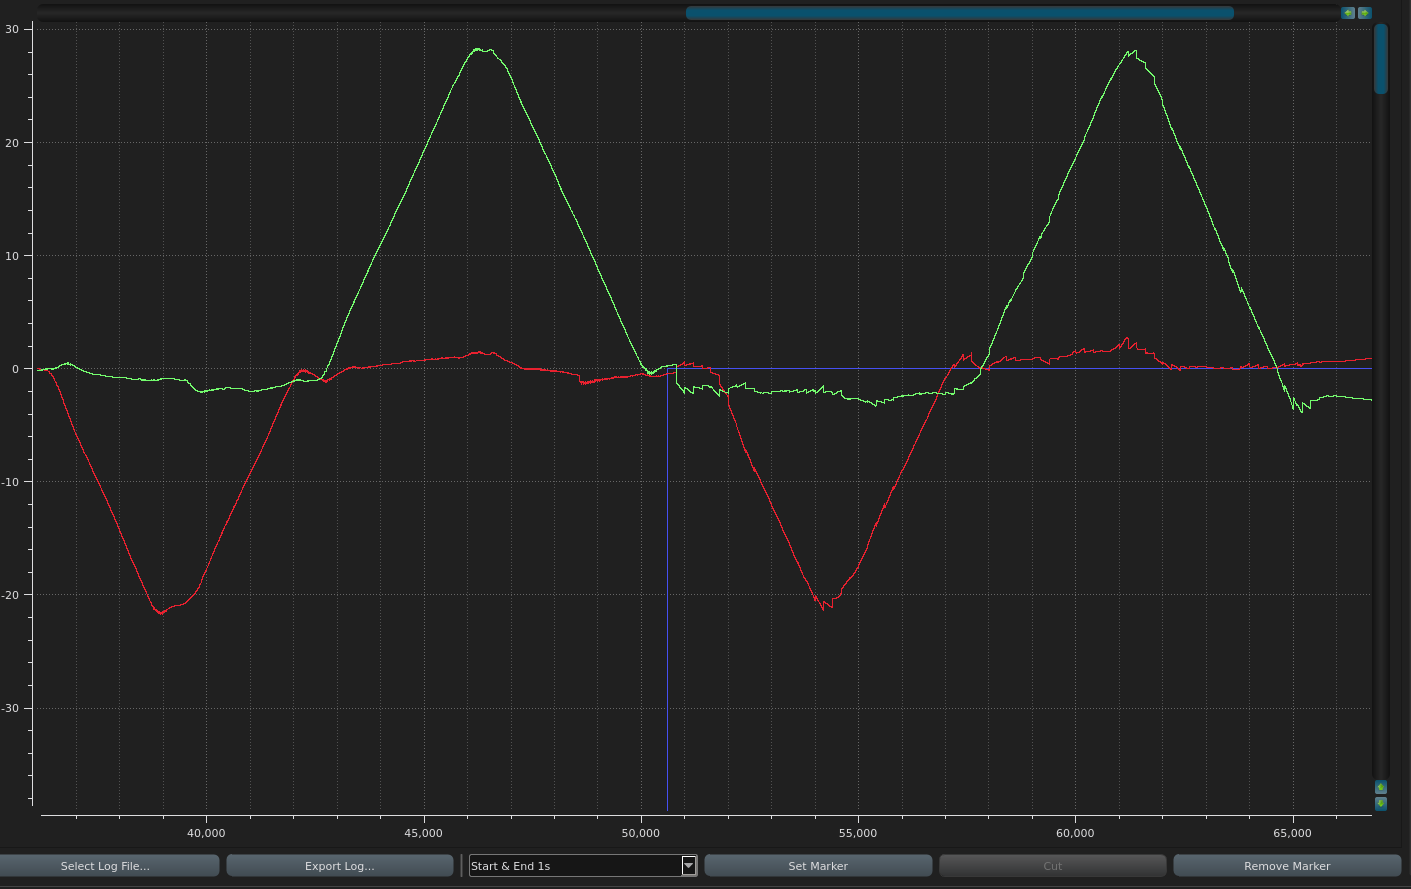
\includegraphics[width=0.8\textwidth]	{graphics/time_vs_nort_east_ch6.png}
	  \caption{Path walked with x-axis as time and y-axis as nort/west. The blue vertical line in the middle of the image shows the switch changing value. Before the blue line is the onboard GNSS used, after the blue line is the NEo-6P used. If looking closely it can be seen the path was walked twice. The read and green line are output from the UKF}
    \label{fig:outdoor_test_walk_90_deg_x_as_time}
\end{figure}

Figure \ref{fig:outdoor_test_walk_90_deg_x_as_time} matches with the walked path seen in figure \ref{fig:outdoor_test_walk_90_deg}. The blue line crossing in the middle is the switch on the Spectrum DX9 transmitter getting activated to switch between the GNSS'. It can be seen how the path repeats itself after the switch has been activated. 
Figure \ref{fig:outdoor_test_zoom_in} shows the same as figure \ref{fig:outdoor_test_walk_90_deg_x_as_time} however vDOP and hDOP has been added to the plot.


\begin{figure}[H]
\centering
    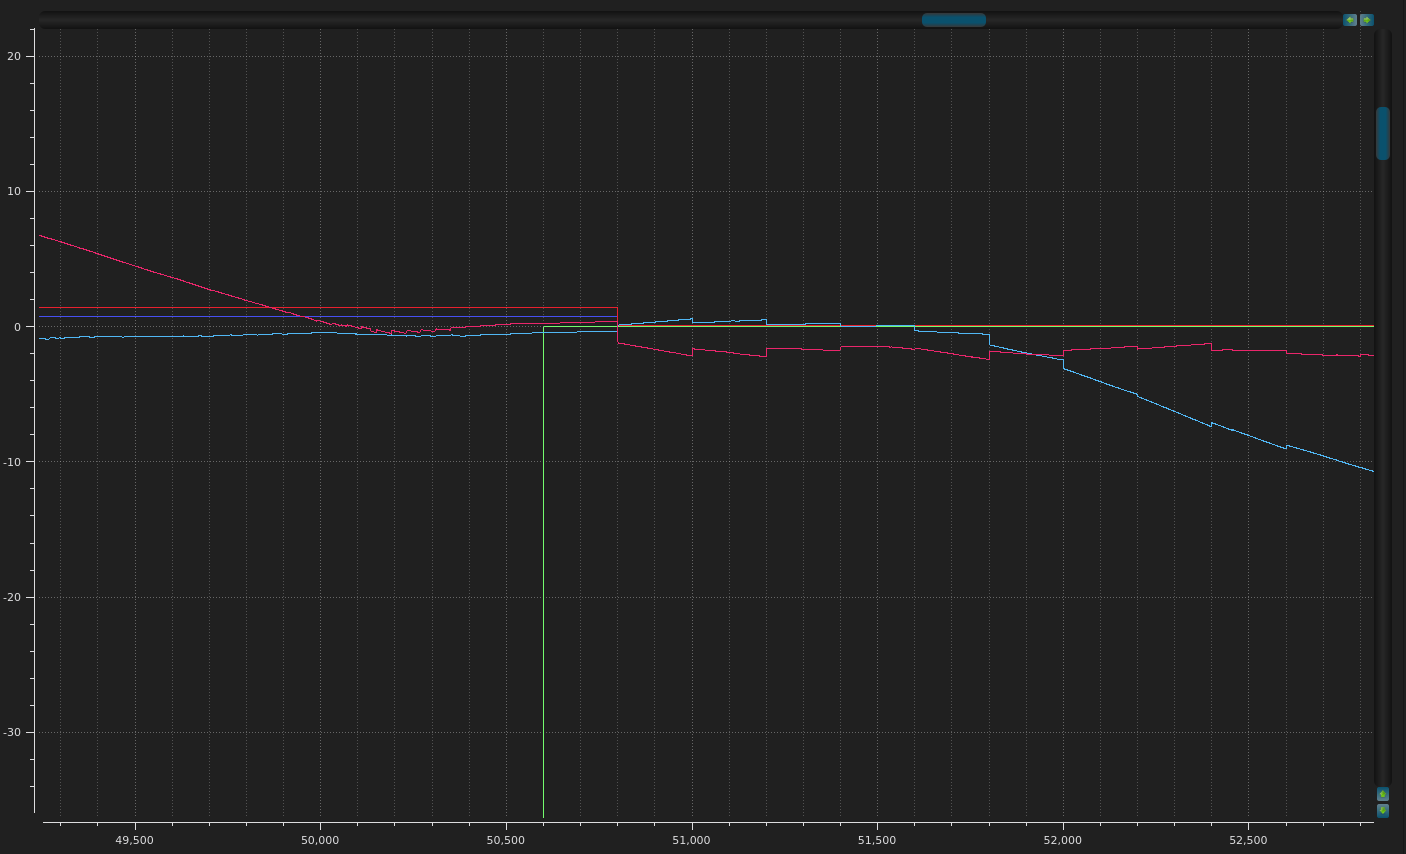
\includegraphics[width=0.9\textwidth]	{graphics/outdoor_test_zoom_in.png}
	  \caption{Figure shows a zoom-in on the GNSS switch. Read is pos-easting, light blue is pos-northing, yellow is switch on transmitter and the two resulting colors are hDOP and vDOP. Note how the position gets less smooth after the GNSS switch. Furthermore, notice how the DOP values decreases when the first GNSS position is received after the switch.}
    \label{fig:outdoor_test_zoom_in}
\end{figure}

Figure \ref{fig:outdoor_test_zoom_in} shows the same plot but where the vDOP and hDOP has been added. It can be seen if looking carefully, how hDOP and vDOP change from ~1 and ~1.5 respectively to ~0. This was due to a divide error in the code. This shows that the belief of the GNSS can be changed by adjusting the DOP values.


\begin{figure}[H]
\centering
    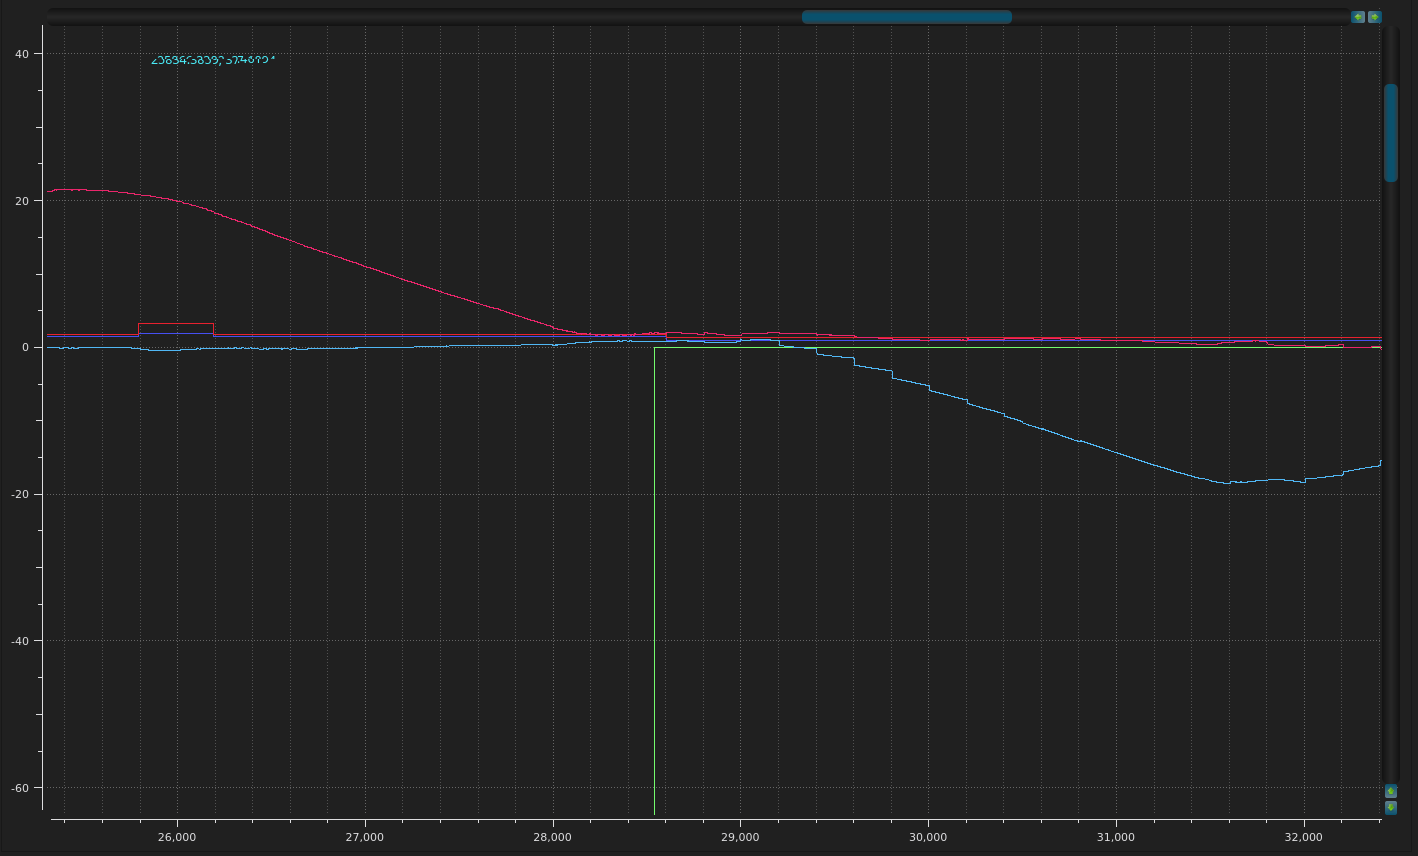
\includegraphics[width=0.9\textwidth]	{graphics/time_vs_north_east_fixed_dop.png}
	  \caption{Figure shows a zoom-in on the GNSS switch. Red is pos-easting, light blue is pos-northing, yellow is switch on transmitter and the two resulting colors are hDOP and vDOP. Notice how the position is more smooth than in figure \ref{fig:outdoor_test_zoom_in}. By inspection in QGroundControl it can be seen the vDOP and hDOP drops ~0.5 from 1.8 and 1.4 respectively which is probably caused by the antenna on the Neo-6P is better}
    \label{fig:outdoor_test_zoom_in}
\end{figure}

It can be seen in figure \ref{fig:outdoor_test_zoom_in} that the UKF performs better when the DOPs are provided correctly.

The velocities was also compared as shown in figure \ref{fig:outdoor_vel_n_vel_e}.
\begin{figure}[H]
\centering
    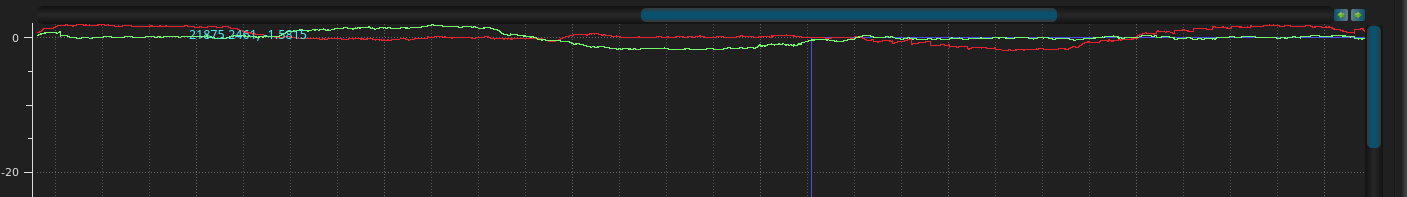
\includegraphics[width=0.9\textwidth]	{graphics/time_vs_vel_n_e.png}
	  \caption{Read line is velocity north, green is velocity east and the vertical blue line shows the GNSS switch. When the switch is zero, the spoofed GPS is used. It can be seen the velocity looks simular, however there exists more ripple on the spoofed GPS}
    \label{fig:outdoor_vel_n_vel_e}
\end{figure}
Figure \ref{fig:outdoor_vel_n_vel_e} shows the velocities with onboard GNSS and Neo-6P GPS. It can be seen there exists some ripple. However it was later discovered that the onboard GNSS provides positions and velocity at 5 hz but the graphs shown aboive is only when the NEo-6p was sending at 1 hz. Unfortunately no log is available with the increased frequency. \footnote{If more time was avaiakble, the 20 meter west, 20 meter north test should be conducted again with 5 hz instead of 1 hz.}

It can be concluded that spoofing the onboard GNSS works over CAN works. The values are compared and it can be seen the two GNSS performs almost equally well. 